\documentclass[runningheads]{llncs}

\usepackage[T1]{fontenc}
\usepackage{graphicx}
\usepackage{hyperref}
\usepackage{amsmath,amssymb}
\usepackage{setspace}
\usepackage{etoolbox}
\usepackage{enumitem}

\newcommand{\ms}[1]{\ensuremath{\mathsf{#1}}}
\newcommand{\msi}[1]{\ensuremath{\mathsfit{#1}}}

\begin{document}

\title{A Decentralized Mnemonic Backup System\\ for Non-Custodial Cryptocurrency Wallets}
\titlerunning{A Decentralized Mnemonic Backup System}

\author{Thierry Sans\inst{1,2} \and
(David) Ziming Liu\inst{2}\and
Kevin Oh\inst{2}}

\institute{University of Toronto Scarborough, Toronto, Canada \and PriFi Labs Inc. Toronto, Canada \\[2ex] \email{thierry.sans@utoronto.ca} \makebox[1em]{} \email{david.liu@prifilabs.com} \makebox[1em]{} \email{kevin.oh@prifilabs.com}}

\maketitle             

\begin{abstract}

When using non-custodial cryptocurrency wallets such as Exodus (Bitcoin), Metamask (Ethereum), and Keplr (Osmosis), the private keys are directly stored on the user's device. Using such a wallet comes with the risk of losing all crypto assets when the device gets lost, stolen, or breaks down irremediably. Fortunately, most non-custodial wallets offer a way to recover the private keys by the mean of a ``recovery phrase'' also known as a ``mnemonic seed phrase''. It is the 12-word phrase that is given when the wallet is created. Indeed, this mnemonic phrase is a really sensitive piece of information since anyone knowing that phrase can get full control of the crypto assets held by the wallet. Usually, it is recommended to write this passphrase down on a piece of paper and store it in a “safe place”. However, storing a physical object is still not ideal since it can get stolen, lost, or destroyed as well. In this paper, we propose a decentralized application that can be used to back up mnemonic phrases and recover them eventually using a simple email. This application is built on a privacy-preserving blockchain to store the confidential passphrase and protect the identity of its owner.

\keywords{Blockchain  \and Smart Contracts \and Decentralized Applications \and Privacy \and Wallets \and Cryptography Protocol}
\end{abstract}

\section{Introduction}

In the world of cryptocurrency, a {\em wallet} provides users with an interface to manage their crypto assets. Under the hood, those wallets store a set of private keys and use them to sign transactions. There are two types of wallets: ``custodial wallets'' in which the private keys are in the custody of a trusted third party and ``non-custodial wallets'' in which the private keys are directly stored on the user's device whether it is a computer, a mobile phone or a dedicated USB dongle. Using either of these types of wallets comes with inherent risks \cite{azar2022financial}. Using custodial wallets comes with the risk of losing all crypto assets when the trusted entity goes bankrupt\footnote{as popularized by the mantra from {\em Andreas Antonopoulos}: {\em ``Not Your Keys, not Your Coins''}} and non-custodial wallets come with the risk of losing all crypto assets if the device gets lost, stolen, or irremediably breaks down. \\

Yet, non-custodial wallets (our focus here) such as Exodus (Bitcoin), Metamask (Ethereum), and Keplr (Secret Network) offer a way to recover the private keys through the mean of a ``recovery phrase'' also known as ``mnemonic seed phrase''. That phrase is usually between 12 and 24 words and it is generated when the user creates the wallet. Here is an example of such a phrase: 

\begin{quote}
\begin{center}
{\tt witch fox practice feed shame open}\\
{\tt despair creek road again ice least}
\end{center}
\end{quote}

That phrase is important as it is used to generate the same private keys on demand (BIP39 standard \cite{palatinus2013mnemonic}). It can be used as a backup or to import the wallet into a new device. Indeed, this mnemonic phrase is a really sensitive piece of information. Anyone who has access to this phrase would have full control over the crypto assets as explained in the {\em Metamask} Wallet FAQ page:

\begin{quote}
{\em ``MetaMask requires that you store your Secret Recovery Phrase in a safe place. It is the only way to recover your funds should your device crash or your browser reset. We recommend you to write it down. The most common method is to write your 12-word phrase on a piece of paper and store it safely in a place where only you have access. Note: if you lose your Secret Recovery Phrase, MetaMask can’t help you recover your wallet. Never give your Secret Recovery Phrase or your private key(s) to anyone or any site, unless you want them to have full control over your funds.''}\\
\end{quote}

As written above, users are not supposed to remember that phrase like a password but instead write it down on a piece of paper and store it in a ``safe place''. However, storing physical objects is still not ideal since they can get stolen, lost, or destroyed as well. As a consequence, users do not always follow such a recommendation and put themselves at risk as studied in \cite{voskobojnikov2021u}. So, as an alternative, could we design a simple application that would take custody of that passphrase and would allow users to recover it based on some sort of authentication? Intuitively, that application could be something similar to a password manager but such a solution requires 1) that the service provider is trustworthy and 2) that the whole application is secured \cite{li2014emperor}. Moreover, a password manager is a centralized solution that goes against the idea of decentralized applications \cite{buterin2017ethereum,cai2018decentralized}.\\

In this paper, we propose a decentralized application that can be used to back up mnemonic phrases protected with a new type of crypto asset, that we call a {\em Passphrase Lock}, that will be distributed to other users. When it is time to recover these mnemonic keys, the user can unlock the passphrase using a simple email. This application is built on a privacy-preserving blockchain \cite{zyskind2015decentralizing} to store the confidential passphrase and protect the address of the Passphrase Lock holders. To better explain our idea, we will go through 3 iterations each more secure than the previous one. In the first iteration (section \ref{iteration1}), we aim at capturing the user experience but its overall design is rather naive and not secure. The attacker can retrieve the passphrase by stealing the user's wallet that was used for backing up the passphrase or by breaching the user's email. We fix those two shortcomings in the second iteration by introducing the concept of {\em Passphrase Lock} and by adding a second layer of encryption to ensure {\em perfect forward secrecy}. Finally, in the third iteration (section \ref{iteration3}), we improve the reliability by distributing the Passphrase Lock to multiple users and recovering the passphrase with only a subset of these users. 

\section{Background}

Our Mnemonic Backup System is a decentralized application developed and deployed on a privacy-preserving blockchain called {\em Secret Network} \cite{zyskind2015decentralizing}. Secret Network Smart Contracts enable storing and processing of private data directly on the blockchain. It relies on the Intel SGX (Software Guard Extension) Trusted Execution Environment (a.k.a Confidential Computing) \cite{mckeen2013innovative} to prevent nodes from reading private data directly from memory during execution. To make sure that nodes protect data during transit, processing, and at rest on the blockchain, each node joining the network has to go through a bootstrap process as explained in \cite{secretnetwork}:

\begin{quote}
{\em ``Before the genesis of a new chain, there must be a bootstrap node to generate network-wide secrets that will empower all the privacy features of the Secret Network chain. When the first node joined the Secret Network, it went through a three-step process. First, the enclave of the bootstrap node generated a remote attestation proof to prove the TEE is genuine. Next, the node generated a random 256-bit number known as the consensus seed. The consensus seed is the most critical part of the Secret Network encryption schema as all other keys and therefore functionality of the protocol are contingent upon secure distribution of this originally generated consensus seed. Using HKDF-SHA256 the consensus seed, in combination with other context-relevant data, derived private keys for the process of registering a new node, I/O encryption, and state encryption. New nodes also use HKDF-SHA256 for key derivation using the original seed or second-generation seeds. Next, the consensus seed is sealed to the disk of the bootstrap node. Finally, the remote attestation proof, the public key for the consensus seed exchange, and the public key for the consensus I/O exchange are all published to the Secret Network genesis.json. Curve25519 is the elliptic curve used for asymmetric key generation and ECDH (x25519) is used for deriving symmetric encryption keys which are used to encrypt data with AES-128-SIV.''}\\
\end{quote}

In the remaining of the paper, we assume that an attacker cannot retrieve data during transport and execution without having the user's private key that was used to encrypt those messages. Moreover, we assume that the attacker cannot decrypt the data stored on the blockchain without getting the node consensus seed sealed with the Intel SGX. That said, it is good to acknowledge that several attacks against Intel SGX have been published in the past few years \cite{gotzfried2017cache,nilsson2020survey,murdock2020plundervolt,biondo2018guard} but those vulnerabilities have been mitigated by Secret Network. \\

\section{Iteration 1: The User Experience}
\label{iteration1}

Alice is a blockchain user that holds crypto assets in her wallet. She would like to have an online backup of her wallet's passphrase in case her device gets lost, stolen, or breaks down irremediably. When that doomsday comes, she would like to recover her passphrase using her email. In our first iteration, the user experience is rather simple: 

\begin{itemize}
    \item {\bf When Alice wants to back up a passphrase}, she visits our Mnemonic Backup website and enters her email. After submitting her information, our application sends her an email with a confirmation code that she must copy onto the webpage along with her passphrase to finalize the backup process. 
    \item {\bf When Alice wants to recover a passphrase}, she visits our Mnemonic Backup website and enters her email. Our application sends her an email with a verification code that she must copy onto the webpage before getting her passphrase back. 
\end{itemize}

This user experience is similar to existing security mechanisms used in traditional web applications where we must make sure that the user is the legitimate owner of the email address used for signing up, signing in (with two-factor authentication enabled), or resetting a password.

\subsection{Architecture}

For this first iteration, we implement our Mnemonic Backup System as a smart contract on the Secret Network that records the passphrase when backing up and restores that passphrase when recovering. However, our secret contract cannot send emails by itself, so we are pairing it with an off-chain Mailer Backend that sends emails to users. So, there are three entities in our system:

\begin{itemize}
    \item {\bf The Frontend Client} is the javascript code running in Alice's web browser that allows to back up and recover passphrases.
    \item {\bf The Backup Contract} is the smart contract that stores users' email and passphrases. The Backup Contract is stored on the blockchain and is executed by one of the Secret Network nodes. The Frontend Client interacts with the Backup Contract by sending messages to one of the Secret Network nodes directly.
    \item {\bf The Mailer Backend} is the off-chain server that sends confirmation/verification codes to users by email. For security reasons, the mailer backend never handles the passphrase. The passphrase is always sent back and forth between Frontend Client (running in the browser) and the Backup Contract (running on the Secret Network)
\end{itemize}

\subsection{The Protocol}

{\bf For backup} (see figure~\ref{it1:backup}), the goal is to verify Alice's email address to eventually store her passphrase. 

\begin{figure}[t]
  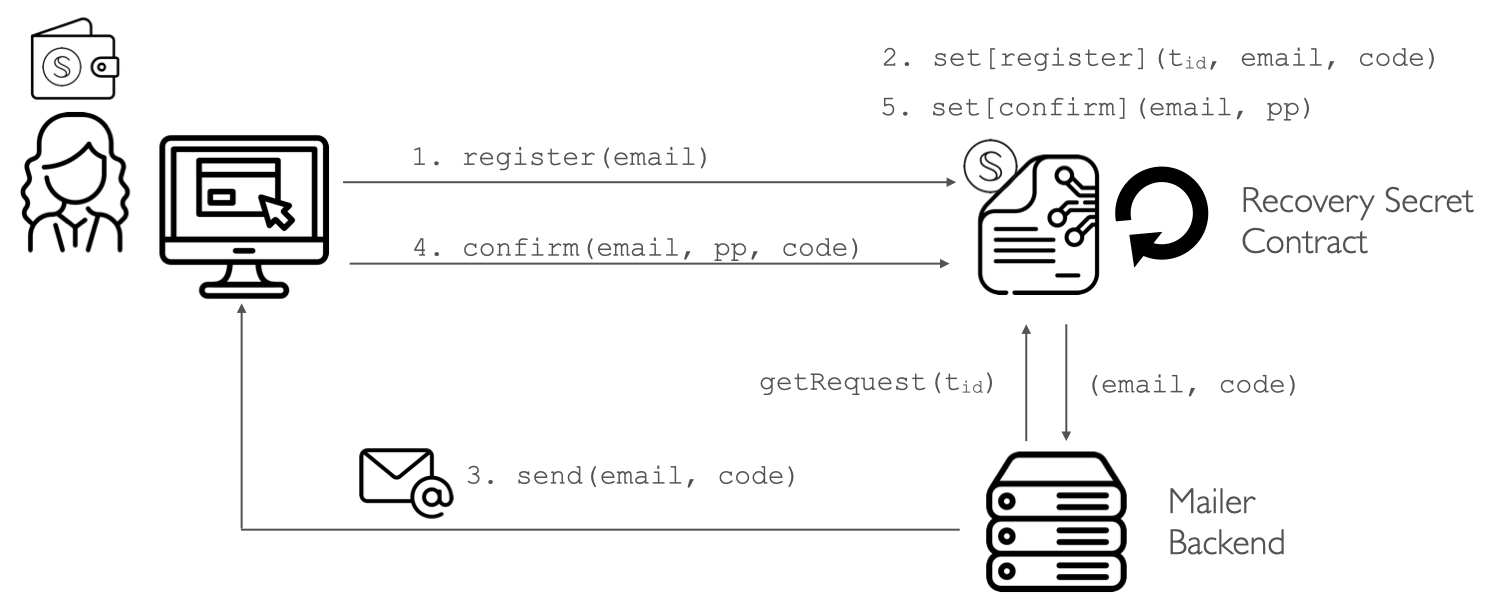
\includegraphics[width=\linewidth]{./media/media-001.png}
  \caption{Iteration 1 - Backup}
  \label{it1:backup}
\end{figure}

\begin{enumerate} 
\item When Alice wants to back up her passphrase, she creates a throwaway wallet (different than the one she wants to back up), provision it, and visits the backup page of the Mnemonic Backup Website. Then, she enters her email and presses the submit button. A script running inside the webpage, called Frontend Client, is executed. The Frontend Client sends a transaction {\bf $\ms{BackupRequest}(email)$} to the Secret Network where a node executes the request using the Backup Contract code. 
\item The Backup Contract generates a transaction id $t_{id}$, a random confirmation code $n$, stores the record $(t_{id}, email, n)$ in the {\tt backup} dataset, and returns the transaction id to Alice.
\item The Frontend Client forwards the transaction id to the Mailer Backend. 
\item The Mailer Backend queries the Backup Contract using that transaction id. 
\item The Backup Contract returns the email and confirmation code $n$ associated to the transaction id. 
\item The Mailer Backend sends the confirmation code to Alice by email. 
\item Alice opens her email and copies and pastes the confirmation code into her browser, and enters her passphrase $pp$. The Frontend Client sends a transaction $\ms{BackupConfirm}(email, pp, n)$ to the Backup Contract. 
\item The Backup Contract verifies the code and stores the record $(email, pp)$ in the {\tt passphrase} dataset. 
\end{enumerate}

{\bf For recovery} (see figure~\ref{it1:recovery}), the goal is to verify Alice's email address to eventually, send her passphrase back. 

\begin{figure}[t]
  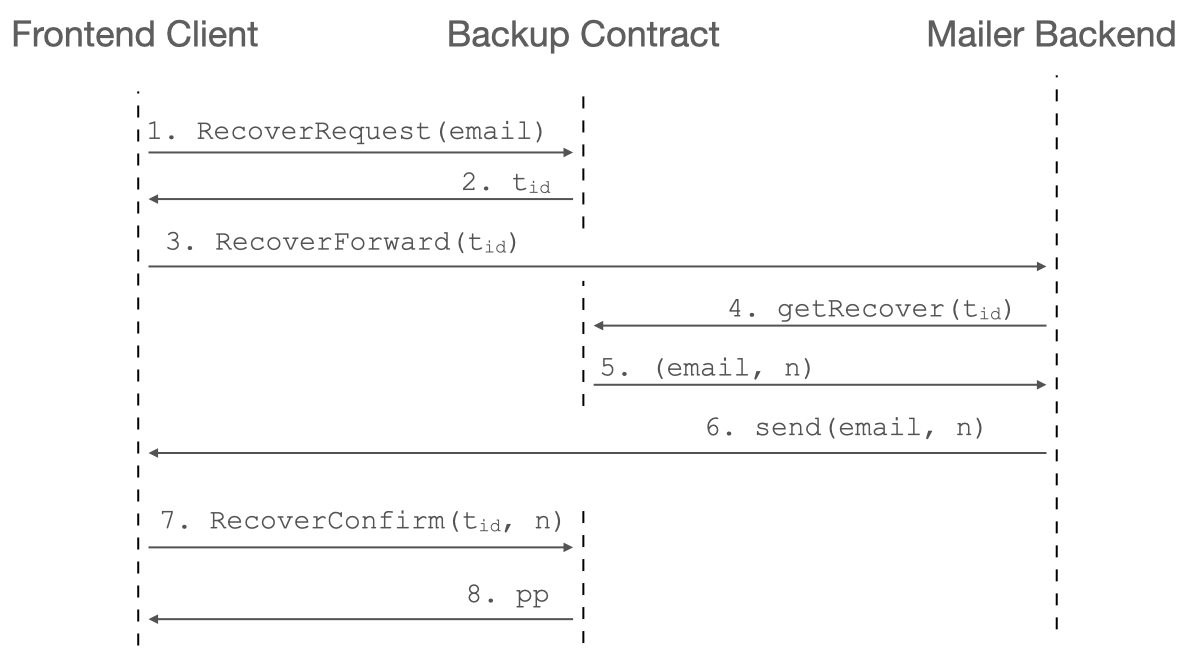
\includegraphics[width=\linewidth]{./media/media-002.png}
  \caption{Iteration 1 - Recovery}
  \label{it1:recovery}
\end{figure}

\begin{enumerate}
\item When Alice wants to recover her passphrase, she creates yet another throwaway wallet (different than the ones she used for backup), provision it, visits the recovery page of the Mnemonic Backup Website and enter her $email$. The Frontend Client (running in the browser) sends a transaction {\bf $\ms{RecoverRequest}(email)$} to the Backup Contract (running on the Secret Network). 
\item The Backup Contract generates a transaction id $t_{id}$, a random confirmation code, stores the record $(t_{id}, email, n)$ in the {\tt recover} dataset, and returns the transaction id to Alice.
\item The Frontend Client forwards the transaction id to the Mailer Backend. 
\item The Mailer Backend queries the Backup Contract using that transaction id. 
\item The Backup Contract returns the email and confirmation code $n$ associated to the transaction id. 
\item The Mailer Backend sends the confirmation code to Alice by email. 
\item Alice opens her email and copies and pastes that verification code into her browser. The Frontend Client sends a query $\ms{RecoverConfirm}(email, n)$ to the Backup Contract. 
\item The Backup Contract verifies the verification code, retrieves the corresponding record from the {\tt passphrase} dataset, and returns the passphrase.
\end{enumerate}

\subsection{Security Analysis}

There are two main security concerns in this first design. First, if the attacker breaches into Alice's mailbox or the Mailer Backend directly, he could retrieve the confirmation code. During the backup phase, the attacker could use the confirmation code to upload an arbitrary passphrase for Alice. This is a problem if Alice recovers what she believes is her original passphrase but another that the attacker can access. Then, any new asset that Alice puts in her wallet can be stolen by the attacker from now. During the recovery phase, it is even worst since the attacker could trigger and use the verification code to query the Backup Contract directly and get the passphrase back. \\

Secondly, if the attacker steals any of the private keys that Alice used for backing up or recovering her passphrase, he could recover the passphrase from the messages. As mentioned earlier, it is recommended that Alice use distinct throwaway wallets when backing up or recovering her passphrase. However, if the attacker steals any of these wallets afterward, he could decrypt the messages stored on the blockchain and recover Alice's passphrase. Said differently, the problem is that our protocol does not ensure the cryptographic property of {\em perfect forward secrecy} \cite{Krawczyk2005}.

\section{Iteration 2: Security Hardening}
\label{iteration2}

Our first iteration captures the right user experience but fails in terms of security. Two main security threats need to be addressed: 1) prevent the attacker from taking advantage of having access to emails and 2) prevent the attacker from recovering passphrases from compromised wallets. We are solving those two problems by introducing a second authentication factor and a second-layer of encryption. 

\subsection{A {\em Passphrase Lock} as a second authentication factor}

The first security problem is an authentication problem. Relying solely on emails to authenticate Alice is insecure if we assume that the attacker could breach Alice’s mailbox, or worse, into the Mailer Backend directly. One way to prevent that is to add a second authentication factor, but this time, we want to rely on the blockchain directly. The idea is for Alice to create a crypto asset called a {\em Passphrase Lock} during backup and transfer that asset to her friend Charlie that will hold that lock. When doomsday comes, Alice should first ask Charlie to transfer the Passphrase Lock back to her before recovering the passphrase. \\

This Passphrase Lock is designed as a crypto asset that Charlie holds in his wallet before eventually transferring it back to Alice's recovery wallet when she needs it. This Passphrase Lock is similar to the concept of NFT \cite{wang2021non} but different in its conception. First, Charlie cannot retrieve Alice's passphrase even if he holds that lock. Moreover, Charlie cannot transfer that crypto asset arbitrarily either. He can only transfer it back to its original owner, Alice, or to any other designated owner approved by Alice. \\

Going back to our original problem, we assume that the attacker can breach Alice's email. However, he would not be able to recover the passphrase without retrieving the Passphrase Lock in his wallet first. In addition, the attacker would not even know who holds Alice's Passphrase Lock since that information is encrypted in the Backup Contract. This is similar to the concept of confidential ownership introduced by Secret Network NFTs in which the owner's address is confidential contrary to other blockchain NFTs. 

\subsection{A second-layer encryption for perfect forward secrecy}

The second security problem comes from the fact that messages sent back and forth between the Frontend Client and the Backup Contract are stored on the blockchain permanently. Unfortunately, these messages can be decrypted afterward by anyone holding the private key that was used to send those messages. This problem can be fixed by adding a second layer of encryption by establishing a session key between the Frontend Client and the Backup contract to encrypt sensitive information sent back and forth. The idea is to use the {\em Diffie-Hellman Key Exchange} protocol to agree on the session key without sharing it explicitly and so preventing it from being stored on the blockchain. That session key is meant to be forgotten as soon as the backup or recovery process is done. \\

The {\em Diffie–Hellman Key Exchange} protocol is a cryptography protocol that allows two parties, usually named Alice and Bob, that have no prior knowledge of each other, to securely agree on a shared key over an insecure channel \cite{diffie2022new}. That channel is considered as insecure because we assume that an attacker can eavesdrop on the communication and read all messages sent back and forth between Alice and Bob\footnote{We only consider message confidentiality here leaving aside authentication and message integrity that is ensured by the Secret Network protocol}. In a nutshell, Alice generates an asymmetric key pair $(sec_A, pub_A)$ and sends the public one to Bob over the in-secure channel. In practice, we use the {\em Elliptic-curve Diffie–Hellman} (abbreviated ECDH) that relies on Elliptic-curve cryptography \cite{bernstein2006curve25519}. When Bob receives Alice's public key, he will also generate its own pair $(sec_B, pub_b)$ and send his public key back to Alice. Once the public keys have been exchanged, Alice and Bob can combine the public key with their private key to generate the same shared secret value $s$. Alice computes $s=\ms{ECDH}(sec_A, pub_A, pub_B)$ and Bob computes the same shared secret value $s=\ms{ECDH}(sec_B, pub_B, pub_A)$. The security of the protocol resides in the fact that an attacker cannot compute that secret value $s$ even if $pub_A$ and $pub_B$ are known but not either $sec_A$ or $sec_B$. In practice, this shared secret value is usually not used as a cryptographic key directly. Instead, that shared value is given as input of a key derivation function such as the HMAC-based extract-and-expand key derivation function $\ms{HKDF}$ \cite{krawczyk2010hmac} that generates the same cryptographic key based on the secret value. 

\subsection{The Protocol}

In addition to the two security measures discussed above, we are also adding additional security measures in both the backup and recovery protocols. First, we check that the request message and the confirm message are sent by the wallet address. Secondly, we limit the time between the request and confirm messages by saving the block Id (denoted $b_{id}$) after the request. Thus the time limit is calculated based on the number of blocks that have been validated between the request and confirm messages.\\

The new {\bf backup protocol} shown in figure~\ref{it2:backup}) goes as such:

\begin{figure}[t]
  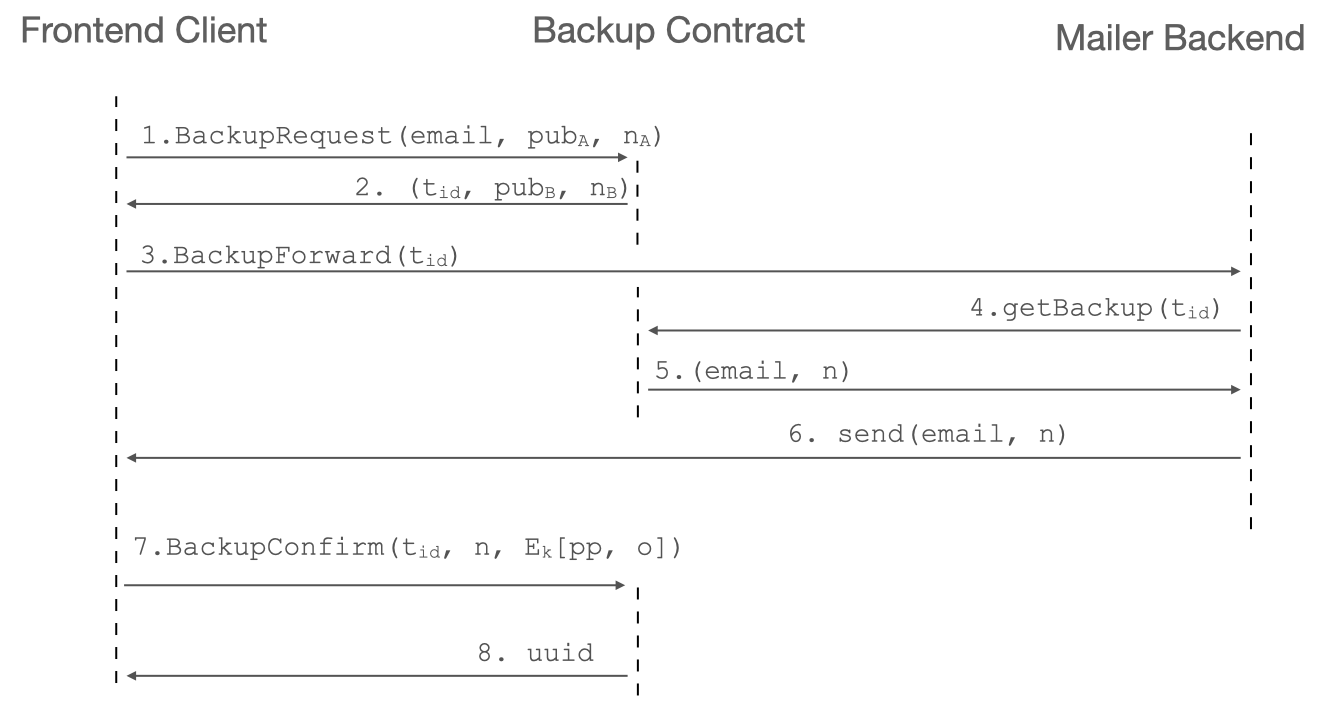
\includegraphics[width=\linewidth]{./media/media-003.png}
  \caption{Iteration 2 - Backup}
  \label{it2:backup}
\end{figure}

\begin{enumerate} 
\item When Alice wants to back up her passphrase, she creates yet a throwaway wallet, provision it, visits the backup page of the Mnemonic Backup website and enters her $email$. The Frontend Client generates an ECDH private and public key pair $(sec_A, pub_A)$, a nonce $n_A$, and sends the transaction $\ms{BackupRequest}(email, pub_A, n_A)$ to Backup Contract.
\item The Backup Contract generates a transaction id $t_{id}$, a new ECDH private and public key pair $(sec_B, pub_B)$, a nonce $n_B$, and returns those values to the client. In addition, the contract calculates the ECDH secret $s=\ms{ECDH}(sec_B, pub_B, pub_A)$, and derives the 128-bit AES symmetric key $k$ using the standard password-based key derivation function $\ms{HKDF}$ and the concatenation of $n_A$ and $n_B$ as a salt $k=\ms{HKDF}(s, n_A || n_B)$. Finally, the contract generates a confirmation code $n$, and stores the record $(t_{id}, email, k, n, @A, b_{id})$ in the {\tt backup} dataset. 
\item The Frontend Client calculates the ECDH secret $s=\ms{ECDH}(sec_A, pub_A, pub_B)$, derives the AES symmetric key $k$ using $\ms{HKDF}$ and the concatenation of $n_A$ and $n_B$ as a salt $k=\ms{HKDF}(s, n_A || n_B)$. Then it forwards the transaction id to the Mailer Backend. 
\item The Mailer Backend queries the Backup Contract $\ms{getBackup}(t_{id})$. 
\item The Backup Contract checks that the query comes from the Mailer Backend wallet's address, retrieves the record from the {\tt backup} dataset, and checks that the query has not expired based on the initial block id $b_{id}$ and the current block id on the Secret Network. If not, it returns the $email$, and the confirmation code $n$ to the Mailer Backend. 
\item The Mailer Backend sends an email to Alice with the confirmation code. 
\item Alice opens her email and copies and pastes the confirmation code into her browser, enters her passphrase $pp$ and the address of Charlie $@C$ that will receive the Passphrase Lock. Finally, the Frontend Client encrypts the passphrase and sends the transaction $\ms{BackupConfirm}(t_{id}, n, E_{k}[pp, @C])$ to the Backup Contract.
\item The Backup Contract checks that 1) the message comes from the same address as the request, 2) the query has not expired based on the initial block id $b_{id}$, and the current block id on the Secret Network and 3) that the confirmation code corresponds to the one stored. Finally, the contract generates a universally unique identifier, stores the record $(uuid, email, pp, @C)$ in the {\tt passphrase} dataset, and returns the $uuid$ back to Alice for the record. 
\end{enumerate}

When Alice wants to recover her passphrase, she creates a new throwaway wallet and contacts her friend Charlie to transfer the Passphrase Lock back to her new recovery wallet following the newly created {\bf transfer protocol} shown in figure~\ref{it2:transfer}):

\begin{figure}[t]
  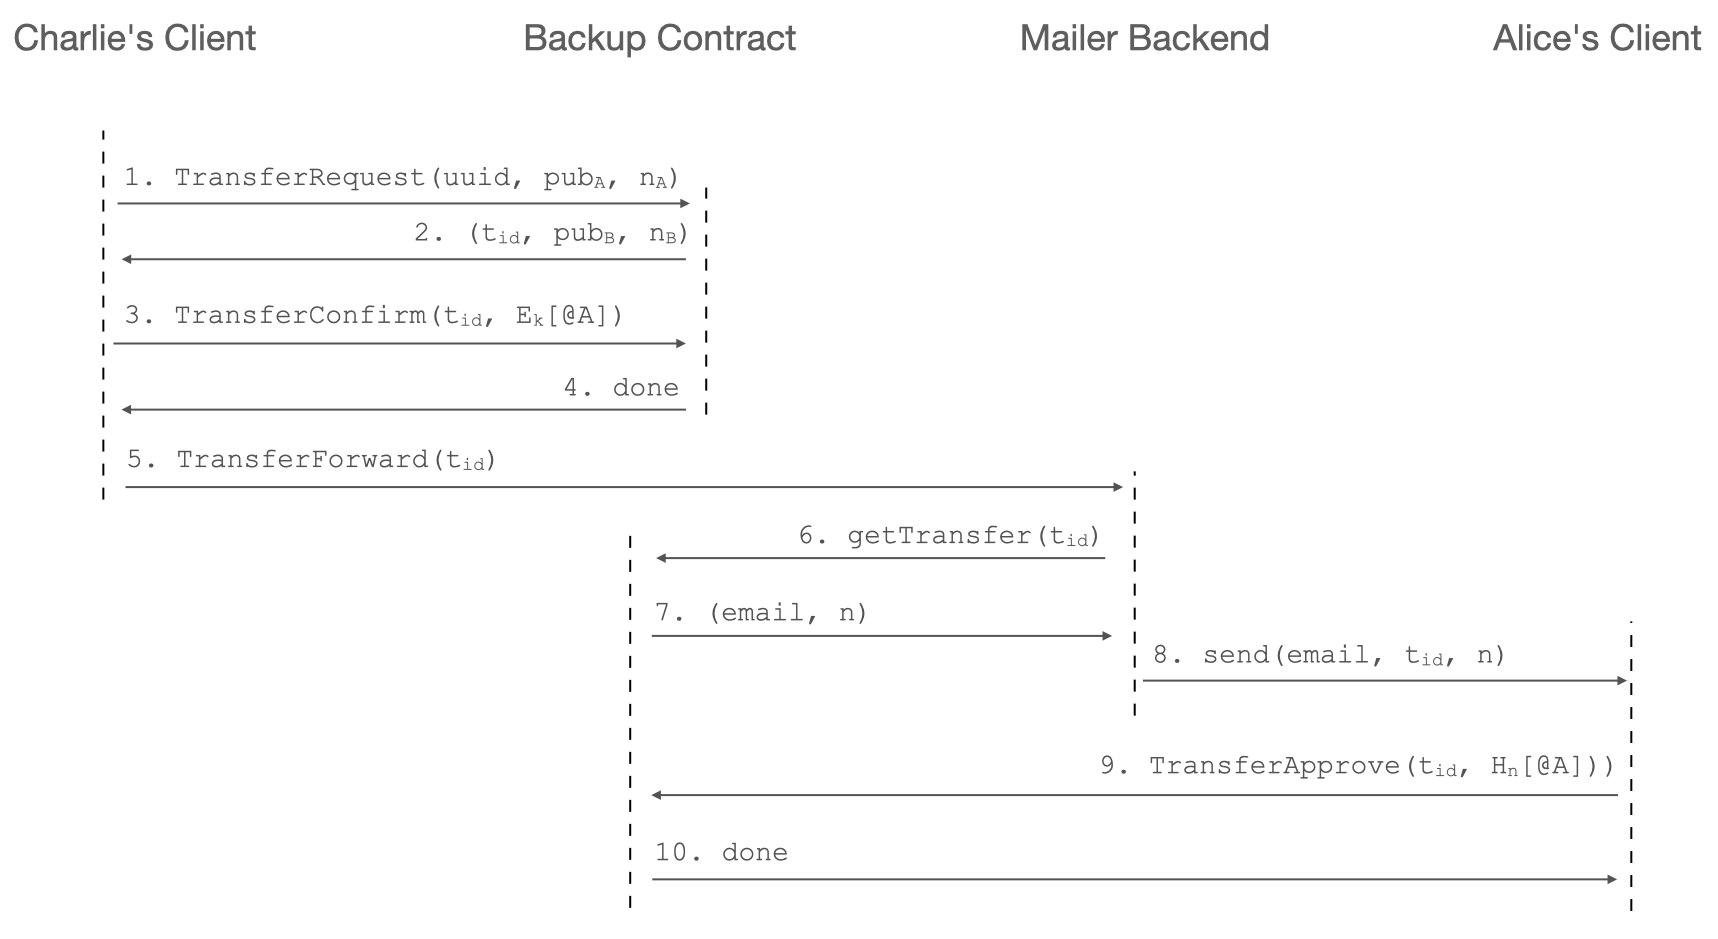
\includegraphics[width=\linewidth]{./media/media-005.png}
  \caption{Iteration 2 - Transfer}
  \label{it2:transfer}
\end{figure} 

\begin{enumerate} 
\item Charlie visits the transfer page of the Mnemonic Backup website and selects the Lock Passphrase to transfer (identified by its $uuid$), enters Alice's new wallet address $@A$ and the password $pwd$. The Frontend Client generates an ECDH private and public key pair $(sec_A, pub_A)$, a nonce $n_A$, and sends the transaction $\ms{TransferRequest}(uuid, pub_A, n_A)$ to the Backup Contract. 
\item The Backup Contract retrieves the record $(uuid, email, pp, @C)$ from the {\tt passphrase} dataset and checks that the Passphrase Lock owner $C$ corresponds to Charlie's wallet address. Then, it generates a transaction id $t_{id}$, a new ECDH private and public key pair $(sec_B, pub_B)$, a nonce $n_B$, and returns those values to the client. In addition, the contract calculates the ECDH secret $s=\ms{ECDH}(sec_B, pub_B, pub_A)$, and derives the 128-bit AES symmetric key $k$ using the standard password-based key derivation function $\ms{HKDF}$ and the concatenation of $n_A$ and $n_B$ as a salt $k=\ms{HKDF}(s, n_A || n_B)$. Finally, the contract generates a confirmation code $n$, and stores the record $(t_{id}, email, k, n, @A, b_{id})$ in the {\tt transfer} dataset. 
\item The Frontend Client calculates the ECDH secret $s=\ms{ECDH}(sec_A, pub_A, pub_B)$, derives the AES symmetric key $k$ using $\ms{HKDF}$ and the concatenation of $n_A$ and $n_B$ as a salt $k=\ms{HKDF}(s, n_A || n_B)$. Then, it encrypts the address of the new owner (Alice's address $@A$ here) and sends the transaction $\ms{TransferConfirm}(t_{id}, E_{k}[@A])$ to the Backup Contract. 
\item The Backup Contract checks that 1) the address use for the confirmation is the same as originally recorded, 2) the query has not expired. If so, it decrypts the owner's address and updates the record in the {\tt backup} dataset.
\item The Frontend Client forwards the transaction id to the Mailer Backend. 
\item The Mailer Backend queries the Backup Contract $\ms{getTransfer}(t_{id})$. 
\item The Backup Contract checks that the query comes from the Mailer Backend wallet's address, retrieves the record from the {\tt transfer} dataset, and checks that the query has not expired. If not, it returns the $email$, the confirmation code $n$ to the Mailer Backend. 
\item The Mailer Backend sends an email to Alice with the confirmation code. 
\item Alice opens her email and copies and pastes the confirmation code, goes to the transfer approval page on the backup mnemonic website, and enters the transfer code and the supposed address of the new owner (Alice's address $@A$ here). The Frontend Client uses the confirmation code to calculate a message authentication code $h$ from the address $h=HMAC_{n}(@A)$. Finally, the Frontend Client sends the transaction $\ms{TransferApprove}(t_{id}, h)$ to the Backup Contract.
\item The Backup Contract checks that the query has not expired. If not, it checks the message authentication from the confirmation code and the address stored in the {\tt transfer} dataset. If there is a match, the {\tt passphrase} record $(uuid, email, pp, @A)$ is updated by changing the ownership of the Passphrase Lock to the new owner's address.
\end{enumerate}

Once the protocol is completed, Alice owns the Passphrase Lock in her new wallet. Now she can use that wallet to recover her passphrase as shown in figure~\ref{it2:recovery}):

\begin{figure}[t]
  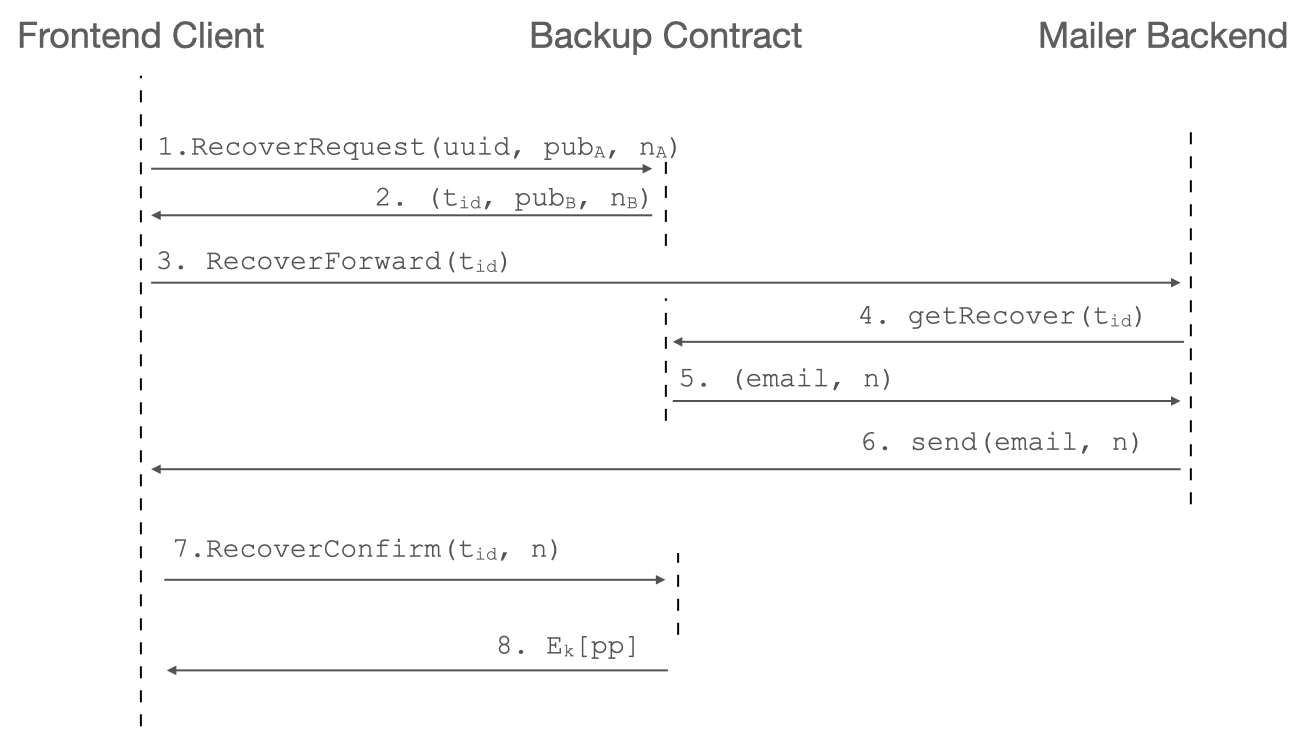
\includegraphics[width=\linewidth]{./media/media-004.png}
  \caption{Iteration 2 - Recovery}
  \label{it2:recovery}
\end{figure}

\begin{enumerate}
\item Alice visits the recovery page of the Mnemonic Backup website and she sees all passphrase records for which she actually hold the lock. She selects the passphrase record she wants to recover (identified by its $uuid$). The Frontend Client generates an ECDH private and public key pair $(sec_A, pub_A)$, a nonce $n_A$, and sends the transaction $\ms{RecoverRequest}(uuid, pub_A, n_A)$ to the Backup Contract.
\item The Backup Contract retrieves the record $(uuid, email, pp, @C)$ from the {\tt passphrase} dataset and checks that the Passphrase Lock owner $A$ corresponds to Alice's wallet address. If so, it generates a transaction id $t_{id}$, a new ECDH private and public key pair $(sec_B, pub_B)$, a nonce $n_B$, and returns those values to the client. In addition, the contract calculates the ECDH secret $s=\ms{ECDH}(sec_B, pub_B, pub_A)$, and derives the 128-bit AES symmetric key $k$ using the standard password-based key derivation function $\ms{HKDF}$ and the concatenation of $n_A$ and $n_B$ as a salt $k=\ms{HKDF}(s, n_A || n_B)$. Finally, the contract generates a confirmation code $n$, and stores the record $(t_{id}, k, pp, email, n, @A, b_{id})$ in the {\tt recover} dataset. 
\item The Frontend Client calculates the ECDH secret $s=\ms{ECDH}(sec_A, pub_A, pub_B)$, derives the AES symmetric key $k$ using $\ms{HKDF}$ and the concatenation of $n_A$ and $n_B$ as a salt $k=\ms{HKDF}(s, n_A || n_B)$. Then it forwards the transaction id to the Mailer Backend. 
\item The Mailer Backend queries the Backup Contract $\ms{getRecover}(t_id)$. 
\item The Backup Contract checks that the query comes from the Mailer Backend wallet's address, retrieves the record from the {\tt recover} dataset, and checks that the query has not expired. If not, it returns the $email$, the confirmation code $n$ to the Mailer Backend. 
\item The Mailer Backend sends an email to Alice with the confirmation code. 
\item Alice opens her email and copies and pastes the confirmation code into her browser. The Frontend Client sends the transaction $\ms{RecoverConfirm}(t_{id}, n)$ to the Backup Contract.
\item The Backup Contract checks that 1) the message comes from the same address as the request, 2) the query has not expired and 3) that the confirmation code corresponds to the one stored. Finally, the contract encrypts the passphrase with the key $k$, and returns it to the client. 
\end{enumerate}

Once the protocol is completed the Frontend Client decrypts the passphrase and displays it to Alice. 

\subsection{Security Analysis}

First, if the attacker can steal any of Alice's private keys afterward, he cannot decrypt the passphrase sent back and forth between the Frontend Client and the Backup contract since the passphrase is always encrypted with the ECDH session key in both the backup and the recovery protocols. In addition, the attacker cannot know the address of Passphrase Lock owner since that information is always encrypted as well. \\

Now, let's assume the attacker has been able to breach Alice's mailbox or the Mailer Backend directly. During the backup, the attacker could get the confirmation code, however, he would not be able to upload an arbitrary passphrase without knowing Alice's private key. For recovery, the attacker cannot initiate the recovery process without first holding the Passphrase Lock. Even if the attacker holds the lock (if the attacker is Charlie for instance), he would not be able to recover the passphrase without also compromising Alice's email. Finally, it takes both the Passphrase Lock owner and the original email owner to work together to transfer the Lock Passphrase. \\

In the end, an attacker cannot retrieve the passphrase without obtaining the lock first {\bf and} compromising the victim's email. \\

However, having a single individual holding Passphrase Lock introduces another problem: what if that person does not or cannot return the Passphrase Lock? The passphrase would be locked forever. We are improving this availability issue in our next and final iteration. 

\section{Iteration 3: Improving Availability}
\label{iteration3}

Having a unique friend holding Alice's Passphrase Lock can be a problem if that friend does not or cannot return it to her. A naive solution would be to duplicate the Passphrase Lock and send it to multiple friends. This solution is feasible but not ideal in terms of security since we are extending the attack surface. The attacker can now target multiple people to regain one of these Passphrase Lock. Instead, our idea is to split the passphrase into multiple parts that we call {\em Passphrase Lock Shares} and send each friend one of these shares. To recover the passphrase, not all shares are needed but a minimum of shares called the {\em threshold}. This is ideal from the usability perspective since the user does not have to collect all the shares back but only the minimum threshold required. Moreover, this is perfect from the security perspective since any attacker who can retrieve any number of shares less than the threshold will not be able to start the recovery process. This approach is similar to threshold cryptosystem such as {\em Shamir's Secret Sharing Scheme} \cite{shamir1979share}. 

\subsection{The Protocol}

The protocol is very similar to the previous iteration with two modifications: 
\begin{itemize}
\item At step 7 in the {\bf backup protocol}, Alice must specify a threshold number $t$, and provide the list of addresses that will receive one {\em Passphrase Lock Share} each. Indeed, the threshold number should be smaller or equal to the number of shareowners. The new backup protocol is shown in figure~\ref{it3:backup}.
\item At step 1 in the {\bf recovery protocol}, the Backup Contract must check that Alice's wallet owns enough Passphrase Lock shares relatively to reach the threshold.
\end{itemize}

\begin{figure}[t]
  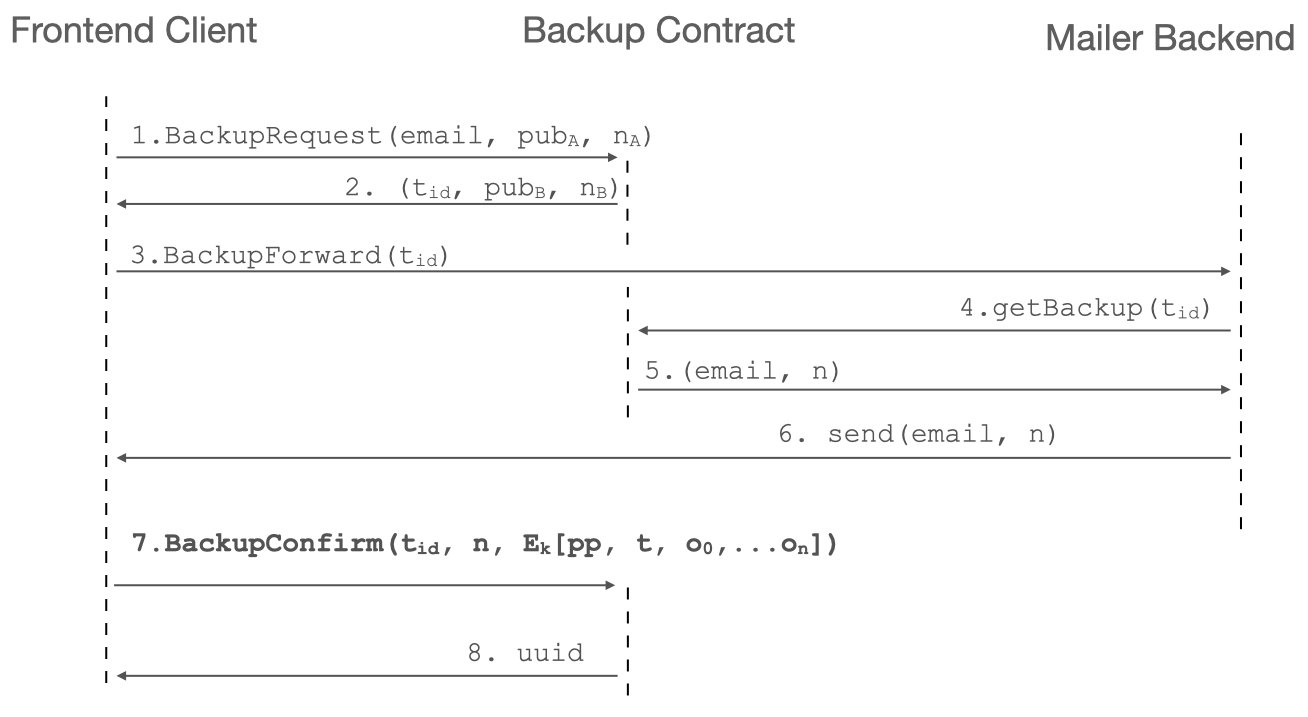
\includegraphics[width=\linewidth]{./media/media-006.png}
  \caption{Iteration 3 - Backup}
  \label{it3:backup}
\end{figure}

\section{Related Work}

Users must keep the wallet's mnemonic phrase safe because whoever gets access to that can access all of the crypto assets held in the wallet. To the best of our knowledge, there is only one significant proposal addressing the same issue. In \cite{rezaeighaleh2019new}, Rezaeighaleh and al. propose using a second wallet for backup. They propose a protocol based on Elliptic-Curve Diffie-Hellman to back up the private keys of the first wallet into a second wallet. They recommend having that secondary wallet be a ``cold'' wallet such as a hardware USB dongle or a smart card. This approach is technically sound but again relies on storing a physical object in a safe place which is hard in practice as shown in \cite{voskobojnikov2021u}. 

\section{Conclusion and Future Work}

In this paper, we propose a Decentralized Mnemonic Backup system that anyone can use to give custody of any blockchain passphrase to a Secret Network smart and protect it using a new type of crypto asset that we call a Passphrase Lock. This Passphrase Lock is split into different shares and distributed to multiple users. When comes the time to recover the passphrase, the user should collect a subset of those shares to unlock the passphrase. \\

The key recovering system can be used outside of our Mnemonic Backup system. It can be used for more advanced cryptographic protocols that involve storing and managing secret keys on-chain with the option of recovering them using an email. For instance, this can be used to encrypt files on the InterPlanetary File System
(IPFS) \cite{muralidharan2019interplanetary} and manage the access using a Secret Contract that would hold custody of the encryption key. Our system could be used to safely generate and manage the encryption key on the Secret Network and possibly have an email backup solution if such a feature is desired.  

\subsubsection{Acknowledgments} This work has been funded through a grant from the {\em Secret Network}.

\bibliographystyle{splncs04}
\bibliography{whitepaper}

\end{document}
